\section{A social player}
\label{sec:social_player}

First of all, a social player in a card game scenario is basically a player that can interact with other human players in a proper way according to the game situation.
Since its behaviours must be as similar as possible to the interactions of human players, the most expressive robot was chosen to embody this player, \ac{emys}.
Nevertheless, when creating behaviours for an embodied agent, it is important to consider that our perception of a social robot, as a unique entity that interact, is indeed composed of distinct modules that make the robot talk, move, animate, gaze at some point or glance at another.
For this reason, the architecture, presented in Figure\ref{fig:model}, uses \emph{Skene} as its \emph{Behaviour Planner}.
\emph{Skene} has its own language, called utterances, that allow the communication with the robot as a single entity.
These utterances are classified with a category and subcategory and may specify verbal or non-verbal behaviours, as well as both interleaved.
Most of \ac{emys} behaviours in this scenario were conducted by \emph{Skene} due to the provided abstraction while producing complete behaviours (verbal and non-verbal), and also due to the utterances classification that can associate behaviours to game states.
The current section will present the main aspects of the utterances list that characterizes \ac{emys} behaviours and the way it will be perceived.
%However, invoking specific instructions without \emph{Skene} can also be directly done

%Additionally, a \emph{Sueca} player has two distinct roles during a game: being partner of his team player and opponent of the other two players.
%With these main concepts in mind, a character of this nature can be developed by specifying its behaviours.
%In other words, considering the connection between the world and the robot is established by \emph{Skene}, this means creating a list of utterances that might contain text to speak, animations, gaze and glance instructions.
%The current section describes the structure of behaviours included in the developed \emph{Sueca} player.


\subsection{\emph{Sueca} behaviours}
The analysis of the card game players on user centred studies revealed key aspects of the interaction during a \emph{Sueca} game.
First of all, there are specific game situations that may cause verbal or non-verbal behaviours.
As a result, these game situations guided the categories and subcategories of the utterances list, presented on the following figure.

\begin{figure}[ht]
	\centering
    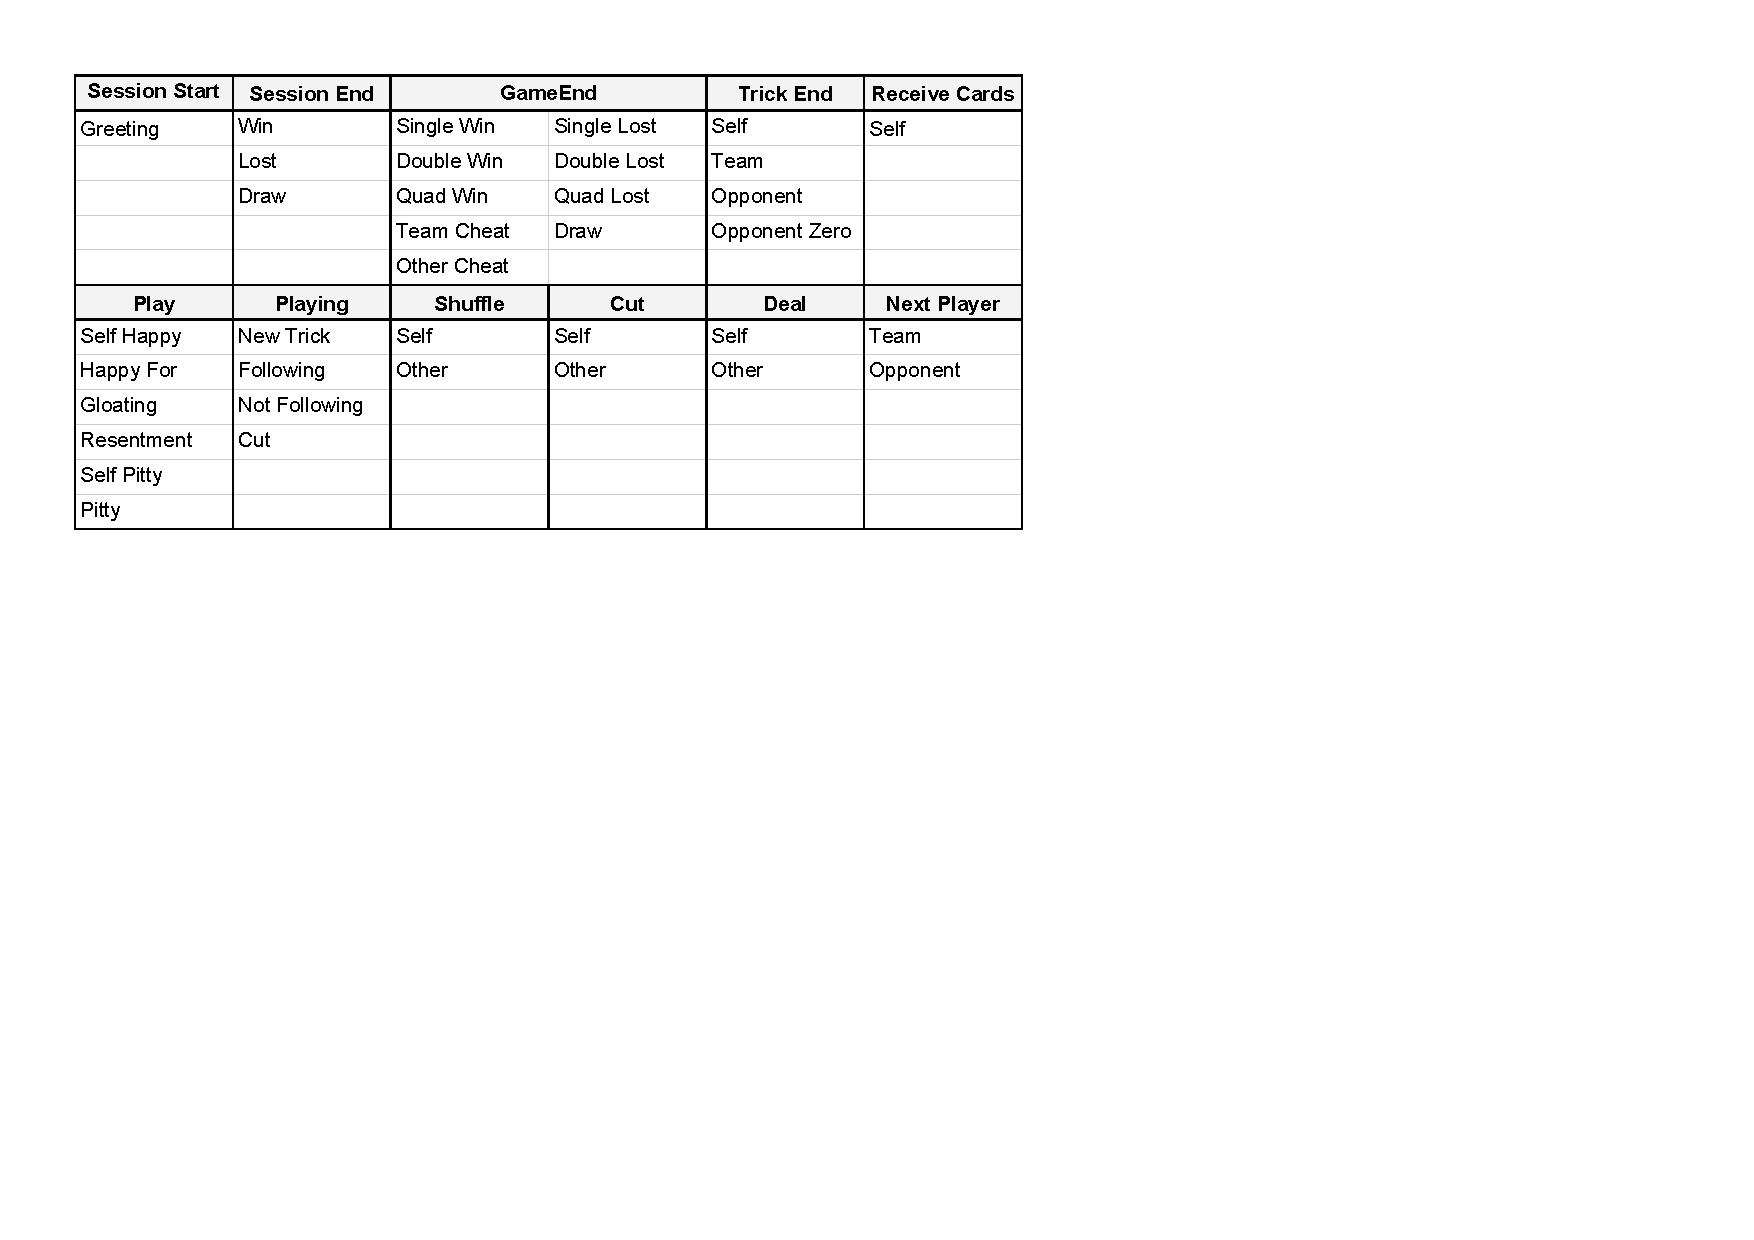
\includegraphics[width=1\textwidth]{./img/utterances}
	\caption{Categories and subtegories of the utterances list}
\label{fig:utterances}
\end{figure}

The final list of 205 distinct utterances was inspired by the collected behaviours and replicated to similar ones in order to enrich interactions and to avoid speech redundancies.
The annotated non-verbal behaviours were also applied on \emph{emys} during the same game situations, for instance, looking at a played card and analysing its own hand after that, simulating a re-evaluation of the game.

\subsection{Human-like behaviours}

Besides simply replicating behaviours from human players, there are other things to consider in order to make the robot act as a human, for instance, its speech frequency or its emotional state.
Consequently, this social player applies a probability to decide whether or not to perform an utterance for each game situation.
Additionally, a \emph{FAtiMA} module was used, as shown in Figure~\ref{fig:model}, to enrich \ac{emys} presence and allow it to share its emotional state.

\emph{FAtiMA} is a modular architecture for an emotional agent capable of producing 22 different emotions based on its goals and its perceptions of new events for a determined scenario.
Perceptions can be updated by changing the values of 6 appraisal variables (desirability, desirability for other, success probability, failure probability, praiseworthiness and like) and their combination can generate one or more emotions.
However, the current emotional agent of this \emph{Sueca} player is only using 4 appraisal variables, which means it only produces 12 emotions, as presented in Figure~\ref{fig:emotions}

\begin{figure}[ht]
	\centering
    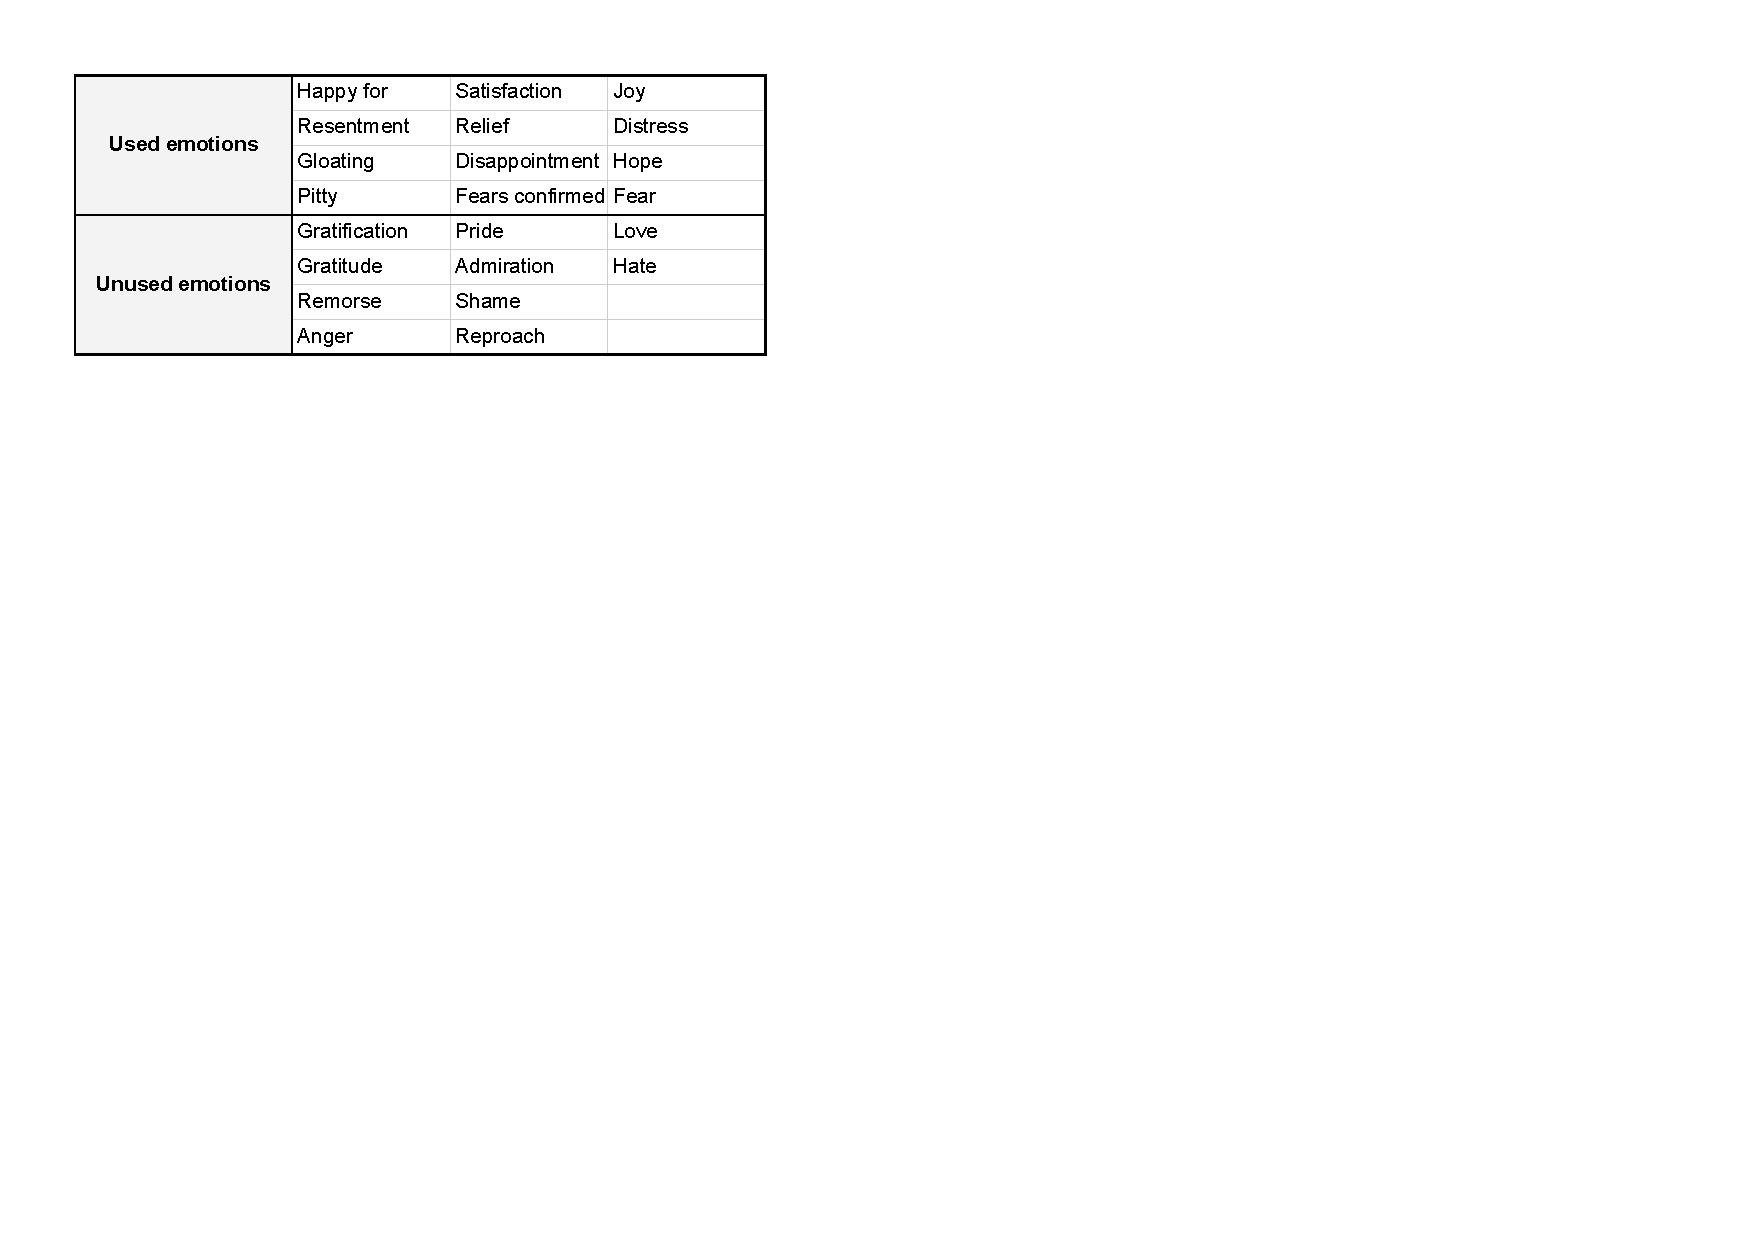
\includegraphics[width=1\textwidth]{./img/emotions}
	\caption{FAtiMA emotions divided}
\label{fig:emotions}
\end{figure}

These emotional states could have been used to subcategorize utterances, however, the analysis of humans playing \emph{Sueca} evidenced their behaviours mostly depend on the specifications of a certain move or simply sign 

frequency
emotions

\subsection{Enhancing the game interface with behaviours}
nextplayer
receiving cards
trick end